\begin{surferPage}[Séptica de Labs]{Uma S\'eptica com 99 Singularidades}
    Oliver Labs construiu uma superf\'icie de grau $7$ (s\'eptica) enquanto trabalhava na sua disserta\c c\~ao na Universidade de Mainz, em 2004. Este \'e o atual recorde mundial para o grau $7$, mas ainda podem existir s\'epticas com um n\'umero de singularidades que pode ascender a $104$.  
    A superf\'icie de Labs tem a simetria de um hept\'agono regular (imagem \`a esquerda).
   Esta propriedade \'e vis\'ivel quando se olha para a superf\'icie a partir de cima (imagem \`a direita):

    \vspace*{-0.3em}
    \begin{center}
      \begin{tabular}{c@{\qquad}c}
        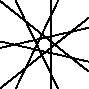
\includegraphics[height=1.5cm]{./../../common/images/labsseptic1.pdf}
        &
        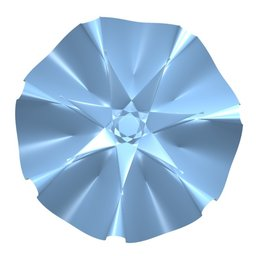
\includegraphics[height=1.5cm]{./../../common/images/labs_septic_von_oben}
      \end{tabular}
    \end{center}
    \vspace*{-0.3em}

    Para construir esta superf\'icie, Oliver Labs utilizou o sistema de \'algebra computacional {\sc Singular} (Universidade de Kaiserslautern),  adequado para c\'alculos em geometria alg\'ebrica e singularidades.

    Labs utilizou o facto de podermos fazer c\'alculos com conjuntos finitos de n\'umeros de um modo natural. Um exemplo deste processo \'e o rel\'ogio: 24.00$=$0.00, 24.00 $+$ 1 hora n\~ao \'e
    25.00, mas sim 1.00.
\end{surferPage}
